\documentclass[handout]{beamer}

\usepackage{fontspec} 
\useoutertheme{lsp}

\usepackage{lsptitle}
\usepackage{booktabs}
\def\two@digits#1{\ifnum#1<10 0\fi\number#1}
\def\mytoday{\two@digits{\number\day}.\two@digits{\number\month}.\number\year}


\usepackage{xspace,multicol}
\newcommand{\latex}{\LaTeX\xspace}
\usepackage{tikz}


\newcounter{lastpagemainpart}
\footnotesep0pt
\renewcommand{\footnoterule}{}
\usefootnotetemplate{
  \noindent
  \insertfootnotemark\insertfootnotetext}

\let\beamerfn=\footnote
\renewcommand{\footnote}[1]{\%
\let\oldfnsize=\footnotesize\%
\let\footnotesize=\tiny\%
\beamerfn<\thebeamerpauses->{#1}\%
\let\footnotesize=\oldfnsize}


\date{\today}

\usepackage{eurosym}  
 
\renewcommand{\centerline}[1]{\hfill#1\hfill\hfill\mbox{}}


\title{\mbox{Community Proofreading}\\
\mbox{\large Zielstellung, Implementation, Evaluation}}
\institute{Language Science Press}
\author[LangSci]{Sebastian Nordhoff}



\begin{document}
\lspbeamertitle

\section{OA $\to$ Open Publishing}

% Um eine widerstandsfähige und tragfähige wissenschaftsgeführte OA-Publikationsplattform wie z.B. Language Science Press aufzubauen und zu betreiben, ist die Einbindung der Community zentral. Nur wenn die Community die Verlagsplattform als "ihre" Plattform annimmt und ihr eine wesentliche Position in der Publikationslandschaft zuschreibt, kann solch eine Plattform längerfristig Bestand haben.
% Eine neuartige Form des Community-Buildings ist das sogenannte Community-Proofreading. Hierbei wird statt eines klassichen Korrektorats die formale Qualitätssicherung an die Leser "crowdgesourct". Einzelne Forscher*innen lesen und korrigieren die Vorabversion je eines Kapitel eines neuen Buches. Hierzu wird die Plattform PaperHive verwendet. Westedt (2018) hat eine erste qualitative Analyse dieses Vorgehens vorgenommen. Ihre Arbeit wird in diesem Vortrag ergänzt um eine quantitative Analyse von über 43.000 Kommentaren von 228 verschiedenen Accounts in insgesamt 52 Büchern, die bei Language Science Press Community-Proofreading durchlaufen haben.
% Hierbei zeigt sich, dass diese Kommentare (unter CC-BY-Lizenz) eine eigene Textsorte darstellen, die Einblicke in psychologische Prozesse beim Lesen und Korrigieren ermöglicht. Die Verwendung einer interoperablen und vernetzten Plattform wie PaperHive mit einer offenen API eröffnet hier ganz neue Nachnutzungsmöglichkeiten von Daten, die im Publikationsprozess bisher eher als Nebenprodukt angesehen wurden. Durch den Verzicht auf eine Gatekeeper-Funktion des Verlages können diese Daten der Wissenschaft zur Verfügung gestellt werden.
% In einer weiteren Analyse wird gezeigt, dass die Autorenbindung durch Community-Proofreading gestärkt wird und dass zukünftige Autoren schon während des Studiums an die "community-eigene" Plattform herangeführt werden.
% Die strikte Trennung der Rollen von Autor*in, Leser*in und Gutachter*in verschwimmt in kollaborativen Prozessen, wie wir sie bei Open-Access-Publikationen finden. Community-Proofreading bildet die stärkere Einbindung der Leserin in den Publikationsprozess ab und leistet so einen wichtigen Beitrag zu community-based/scholar-led Publishing.

\frame{
\frametitle{Open Publishing}
%   \includegraphics[height=.6\textheight]{./path/to/graphicsfile}
  \begin{itemize}
    \item im Open Access geht es meistens um Zugang, d.h. ums Lesen
    \item Open Publishing geht darüber hinaus: 
    \begin{itemize}
      \item Open source platforms 
      \item Open formats 
      \item Open protocols
      \item Open bookkeeping 
      \item Open peer review
      \item \textbf{Community proofreading}
    \end{itemize}    
  \end{itemize}
}

\section{Community}
\frame{
\frametitle{Bibliodiversität}
\begin{columns}
%   \begin{column}{3cm}
%   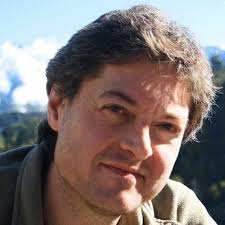
\includegraphics[height=.6\textheight]{mounier.jpg}
%   \end{column}
\begin{column}{7cm}
  \begin{itemize}
    \item Forschende nehmen je nach Uhrzeit ganz verschiedene Rollen ein
    \begin{itemize}
      \item Autor, Gutachterin, Leserin
    \end{itemize}
    \item je jünger desto Leser
    \item je älter desto Gutachter
    \item komplexes Ökosystem
    \item Integration aller Ebenen im community-based Publishing
  \end{itemize}
  \end{column}
\end{columns}
}




\section{Community proofreading}
\frame{
\frametitle{Traditionalles Lektorat/\newline Korrektorat}
\begin{columns}
  \begin{column}{5cm}
  \begin{itemize}
    \item eingekaufte Dienstleistung
    \item 1 Person
    \item spezialisiert in Stil und Richtlinien
    \item fachlicher Hintergrund möglich aber nicht zwingend 
    \item normalerweise kein Spezialwissen in spezifischen Teilgebieten der Linguistik
  \end{itemize}
  \end{column}
  \begin{column}{5cm}
  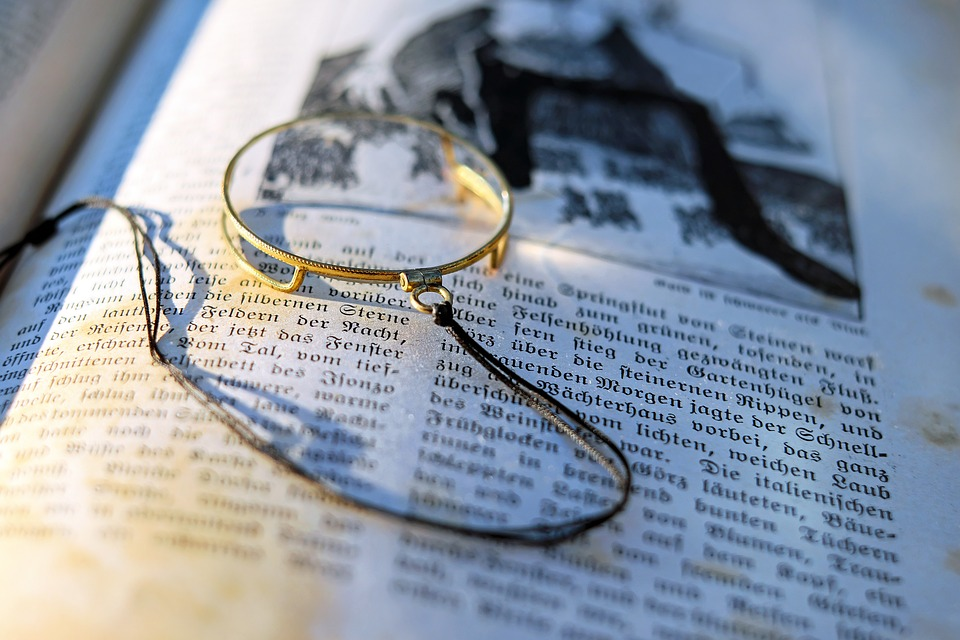
\includegraphics[height=.6\textheight]{lektor.jpg}
  \end{column}
\end{columns}
}



\frame{
\frametitle{Language Science Press}
%   \includegraphics[height=.6\textheight]{./path/to/graphicsfile}
  \begin{itemize}
    \item  Open-Access-Verlag in der Sprachwissenschaft
    \item 100+ Bücher seit 2014 
    \item 350 Community Proofreader
  \end{itemize}
}

\frame{
\frametitle{Katalog}
  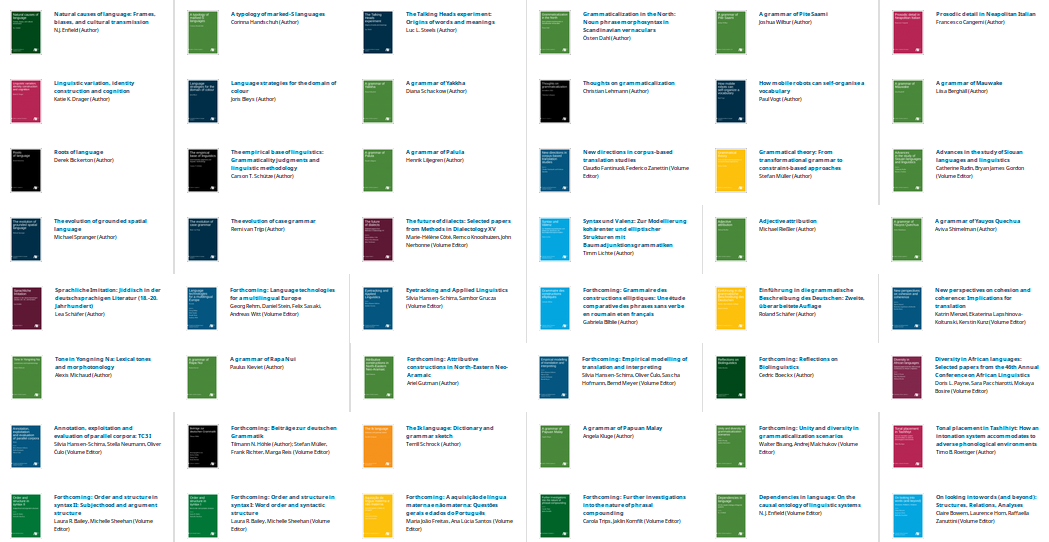
\includegraphics[height=\textheight]{catalog.png}
}

\frame{
\frametitle{Community proofreading}
  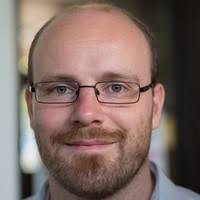
\includegraphics[height=1.5cm]{hoelzl.jpg}~~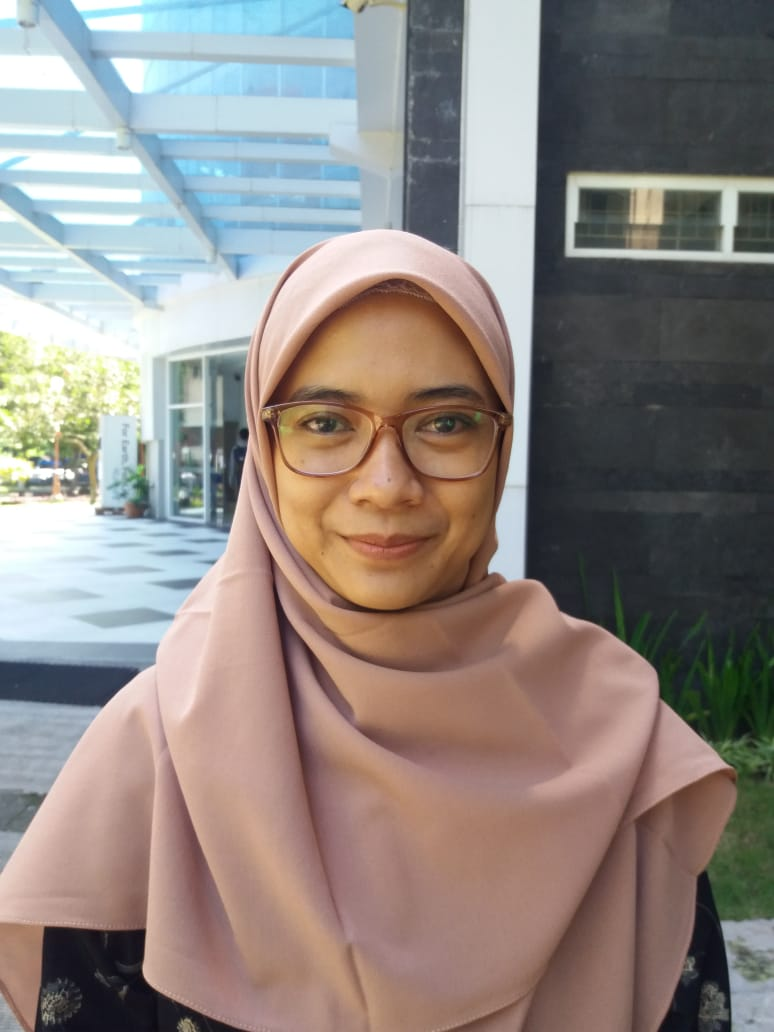
\includegraphics[height=1.5cm]{oktavianti.jpg}~~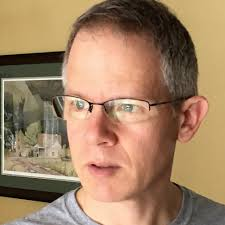
\includegraphics[height=1.5cm]{reynolds.jpg}~~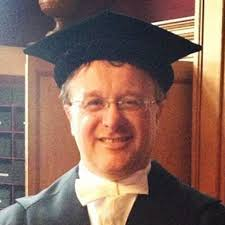
\includegraphics[height=1.5cm]{vandeweijer.jpg} 
  \begin{itemize}
    \item Crowdsourcing
    \item freiwillig
    \item viele Korrektoren, häufig jünger
    \item sehr häufig spezialisiert im Teilgebiet
    \item intrinsisches Interesse
    \item relativ gesehen geringere Expertise in Stilistik und Richtlinien
  \end{itemize}
  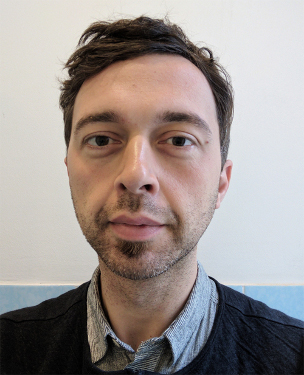
\includegraphics[height=1.5cm]{Doehler.jpg}~~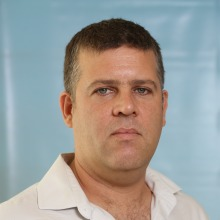
\includegraphics[height=1.5cm]{grossman.jpg}~~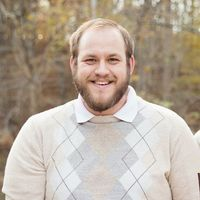
\includegraphics[height=1.5cm]{brinkerhoff.jpg}~~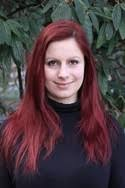
\includegraphics[height=1.5cm]{nitzke.jpg}
}

\frame{
\frametitle{Workflow}
  \begin{itemize}
    \item Proofreading Queue: neuer Titel alle 2 Wochen
    \item Titel wird montags angekündigt
    \item Interessierte können sich für ein Kapitel melden
    \item Kapitel werden mittwochs zugewiesen
    \item Dauer: 4 Wochen
    \item Software: Paperhive
  \end{itemize}
}

\frame{
\frametitle{Paperhive}
  
\includegraphics[width=\textwidth]{paperhive.png}
}

\section{Study}
\frame{
\frametitle{Westedt (2018)}
\begin{itemize}
  \item 
Westedt hat in ihrer BA-Arbeit eine Stichprobe von Kapiteln hinsichtlich der Kommentare analysiert:
\end{itemize}

\centering 
\begin{tabular}{lr}
Kategorie & \%\\
\midrule 
Stil&21.00\\
Wortwahl&20.73\\
Zeichensetzung&11.81\\
Grammatik&11.55\\
Referenzen&9.71\\
Satzbau&7.80\\
Rechtschreibung&7.30\\
\textbf{Inhalt}&\textbf{6.56}\\
Sonstiges&3.41\\
\end{tabular}
}


\frame{
\frametitle{Quantitative Analyse}
%   \includegraphics[height=.6\textheight]{./path/to/graphicsfile}
  \begin{itemize}
    \item nach der qualitativen Analyse Westedts jetzt eine quantitative Analyse
    \item  52 Bücher (2016--2018)
    \item Paperhive-Kommentare wurden per API in eine Datenbank überführt
    \item 19\,004 pdf-Seiten
    \item 43\,370 Kommentare
    \item Datenbasis verfügbar auf \url{https://doi.org/10.5281/zenodo.3063004}
  \end{itemize}
}

\section{Statistik}
\frame{
\frametitle{Länge der Bücher}
  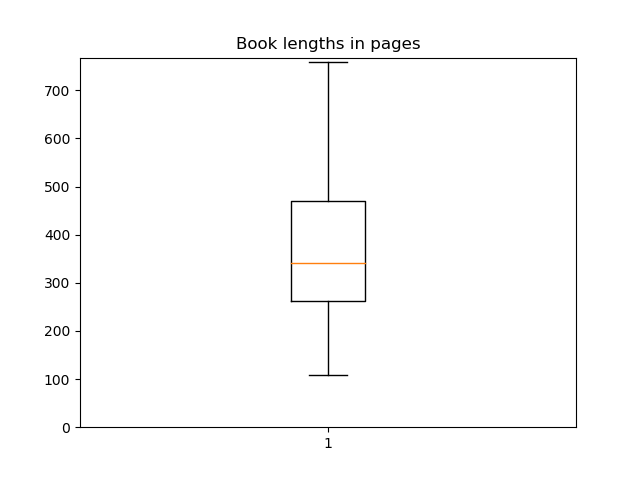
\includegraphics[height=\textheight]{booklengths.png}
}

\frame{
\frametitle{Menge Kommentare}
  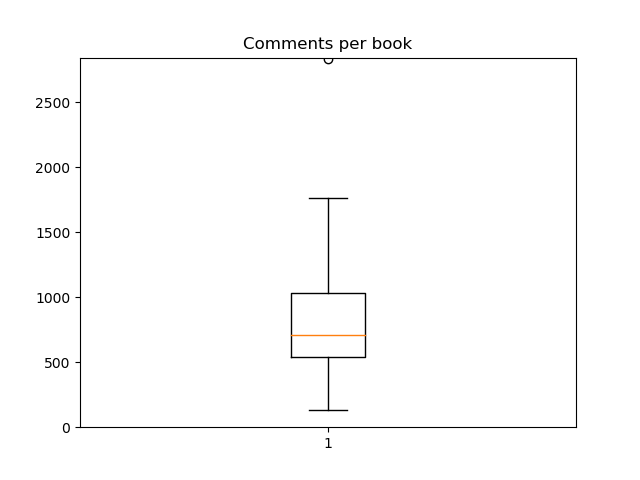
\includegraphics[height=.6\textheight]{commentsperbook.png}
  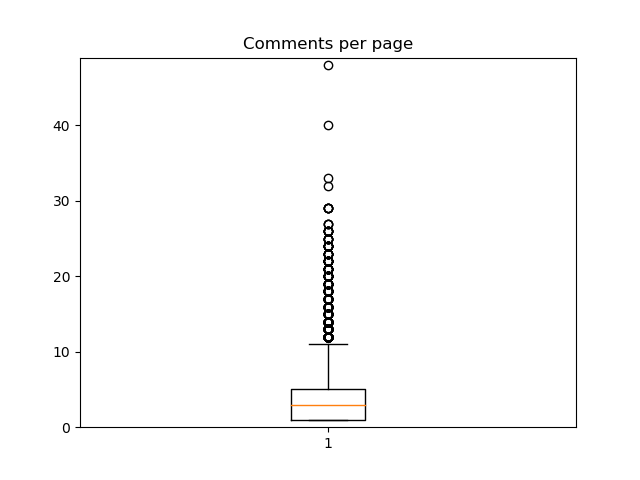
\includegraphics[height=.6\textheight]{commentsperpage.png}
  Die höchste Anzahl Kommentare auf einer Seite findet sich auf Seite 122 von  \textit{Theory and description in African Linguistics} (48 Kommentare).
}

\frame{
\frametitle{Proofreader}
  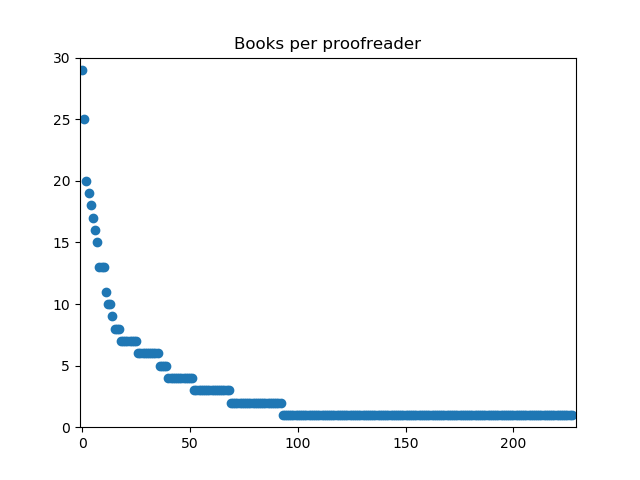
\includegraphics[height=.6\textheight]{booksperproofreader_p.png}
  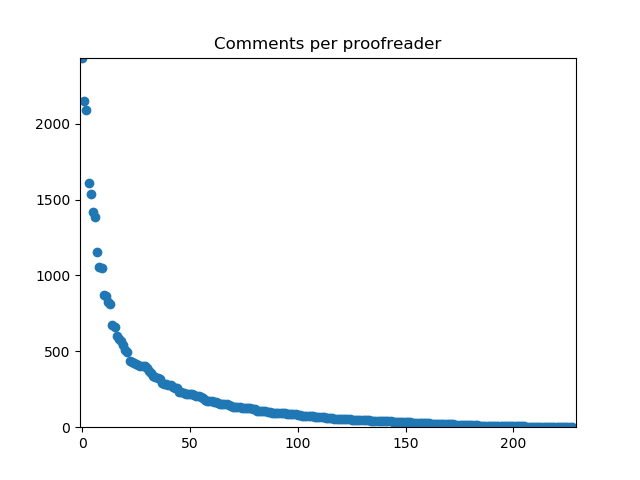
\includegraphics[height=.6\textheight]{commentsperproofreader_p.png}
228 verschiedene Accounts haben bisher am Community Proofreading teilgenommen. 
}

\frame{
\frametitle{Proofreader pro Buch}
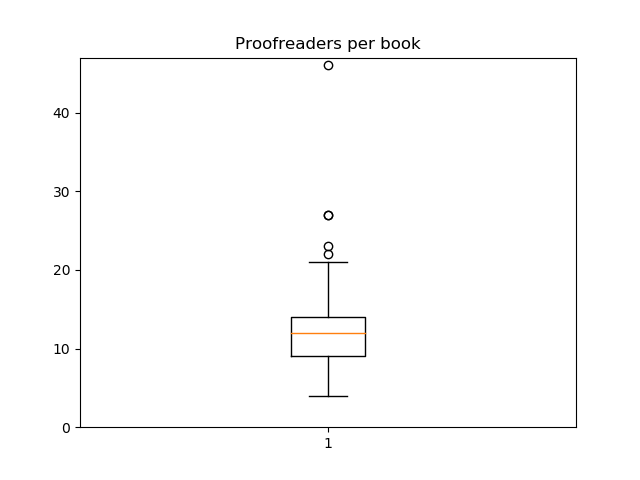
\includegraphics[height=\textheight]{proofreadersperbook.png}
  }

\frame{
\frametitle{Textanalyse der Kommentare}
  
\includegraphics[width=\textwidth]{commenttitlebody.png}
  \begin{itemize}
    \item  Kommentare auf PaperHive haben einen Titel (<40 Zeichen)
    \item zusätzliche Ausführungen in Freitextfeld optional möglich. 
  \end{itemize}
}

\frame{
\frametitle{Title length and body length}
  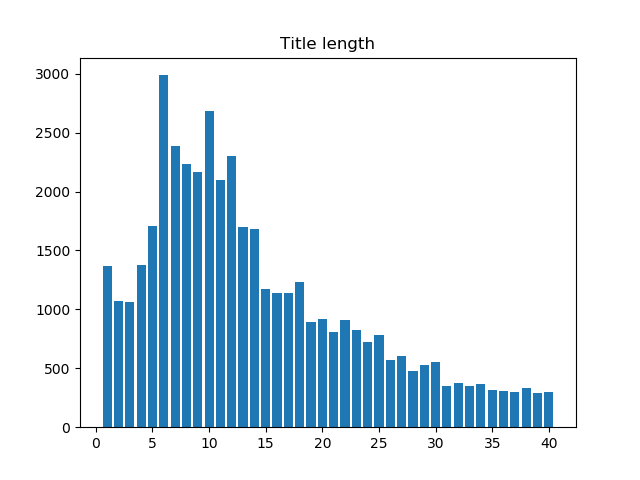
\includegraphics[height=.6\textheight]{titlelength_b.png}
  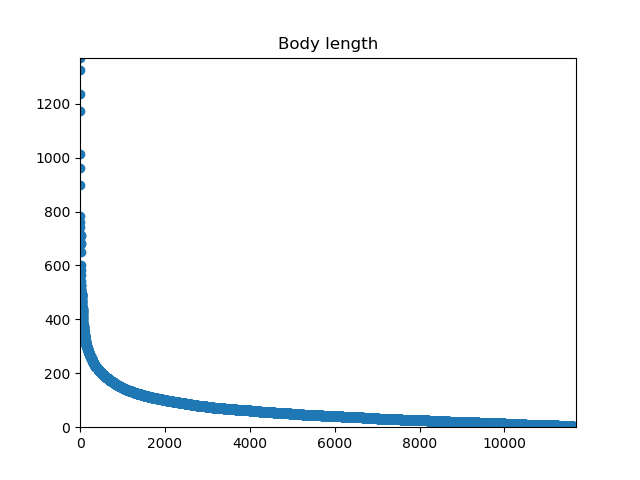
\includegraphics[height=.6\textheight]{bodylength_p.png}
}

\section{Hypothesen}
\frame{
\frametitle{Forschungsfragen an die Daten}
%   \includegraphics[height=.2\textheight]{./path/to/graphicsfile}
  \begin{itemize}
    \item Community Proofreading liefert einen Datensatz an Kommentaren von beträchtlicher Größe und Güte
    \item  Anhand des Datensatzes können verschiedene Hypothesen getestet werden
  \end{itemize}
  
%   \includegraphics[height=.6\textheight]{./path/to/graphicsfile}
  \begin{enumerate}
    \item \textbf{Proofreader fallen in zwei Klassen: Typ 1 konzentriert sich auf kleine Details; Typ 2 sieht das Werk als Ganzes}
    \item \textbf{Kommentare werden gegen Ende des Kapitels kürzer (Ermüdung, Verweise auf vorher Gesagtes)}
  \end{enumerate}
}
 
\frame{
\frametitle{Hypothese 1:\\ 2 Klassen}
%   \includegraphics[height=.6\textheight]{./path/to/graphicsfile}
  \begin{itemize}
    \item  
Typ 1: viele Kommentare, dafür kurz (``comma missing'')
    \item 
    Typ 2: wenige Kommentare, dafür ausführlicher
  \end{itemize}
} 

\frame{
\frametitle{Berechnung}
%   \includegraphics[height=.6\textheight]{./path/to/graphicsfile}
  \begin{itemize}
    \item Für jedes Buch
    \begin{itemize}
      \item 
    ordne alle Teilnehmer nach Menge an Kommentaren
    \item ordne alle Teilnehmer nach durchschnittlicher Kommentarlänge
    \item trage beide Rangordnungen gegeneinander ab
    \end{itemize}
  \end{itemize}
}

\frame{
\frametitle{Beispielplot\\ for Hypothese 1}
  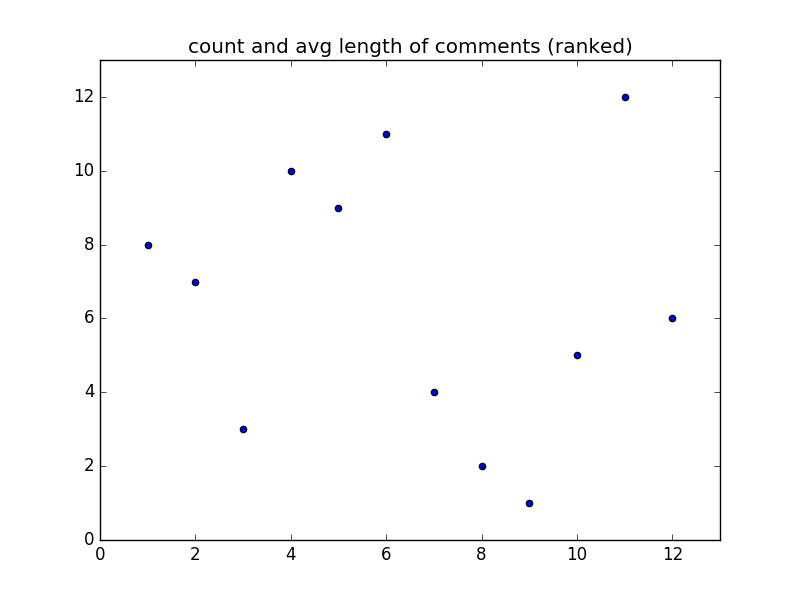
\includegraphics[height=.6\textheight]{allscatterx.png}
\begin{itemize}
  \item 12 Teilnehmer
  \item Rangfolge wird durch Punkte angegeben. 
  \begin{itemize}
    \item e.g. \#3 in Menge ist auch \#3 in Durchschnittslänge, aber \#1 entspricht \#8
  \end{itemize}
  \item Daten eines Buches offensichtlich nicht ausreichend.
\end{itemize}

  }

\frame{
\frametitle{Kombination aller Bücher}
  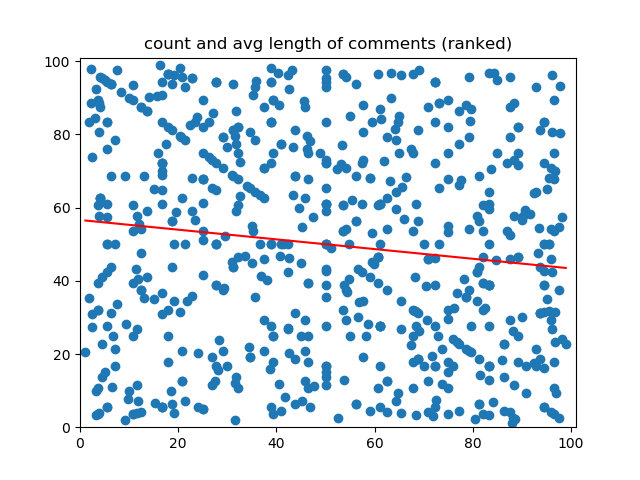
\includegraphics[height=.6\textheight]{allscatter.png}
  \begin{itemize}
    \item Ränge auf Perzentile normalisiert
    \item Rote Linie gibt best fit an
    \item in der Tat eine schwache negative Korrelation
  \end{itemize}
}
\frame{
\frametitle{Ergebnis Hypothese \#1}
%   \includegraphics[height=.6\textheight]{./path/to/graphicsfile}
  \begin{itemize}
    \item Hypothese \#1 bestätigt
    \begin{itemize}
      \item Proofreader mit mehr Kommentaren haben kürzere Kommentare
      \item Proofreader mit längeren Kommentaren haben weniger Kommentare
    \end{itemize}
  \end{itemize}
}


\subsection{Proofreader fatigue}
\frame{
\frametitle{Hypothese \#2:\\ Ermattung}
%   \includegraphics[height=.6\textheight]{./path/to/graphicsfile}
\textbf{Hypothese 2: Kommentare werden mit zunehmender Dauer der Korrektur kürzer, einerseits durch Ermattung, andererseits durch Verweise auf weiter oben Gesagtes.}
}

\frame{
\frametitle{\mbox{Berechnung Hypothesis \#2}}
%   \includegraphics[height=.6\textheight]{./path/to/graphicsfile}
  \begin{itemize}
    \item for every book \\
     ~for every proofreader\\ 
       ~~for every comment
        \begin{itemize}
          \item ermittle relative Kommentarlänge in Prozent (zB 67\% der durschnittlichen Kommentarlänge)
          \item ermittle relative Kommentarposition (vorne, mitte, hinten) in Prozent
          \item trage die Ergebnisse gegeneinander ab
        \end{itemize}
        \item Ein Punkt (0.5, 5) bedeutet, dass der Kommentare in der Mitte des Kapitels 500\% der Durchschnittslänge hatte.
        \item Die relative Position kann anhand der Seiten oder anhand der gereihten Kommentare ermittelt werden
    \end{itemize}
}

\frame{
\frametitle{Plot für Hypothese \#2\\ nach gereihten Kommentaren}
  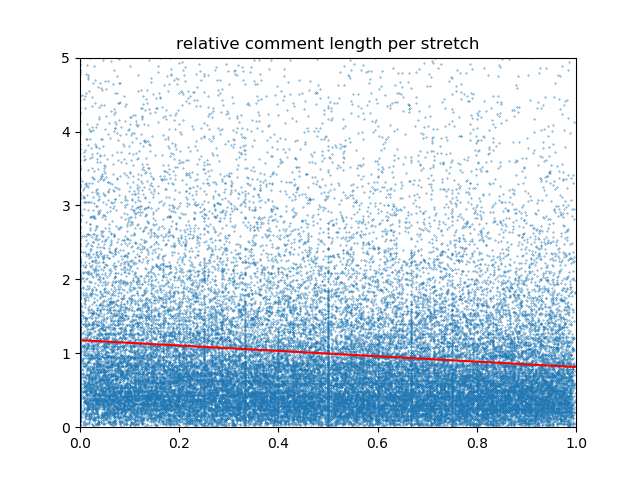
\includegraphics[height=\textheight]{stretches.png}
}

\frame{
\frametitle{Plot für Hypothese \#2\\ nach Seiten}
  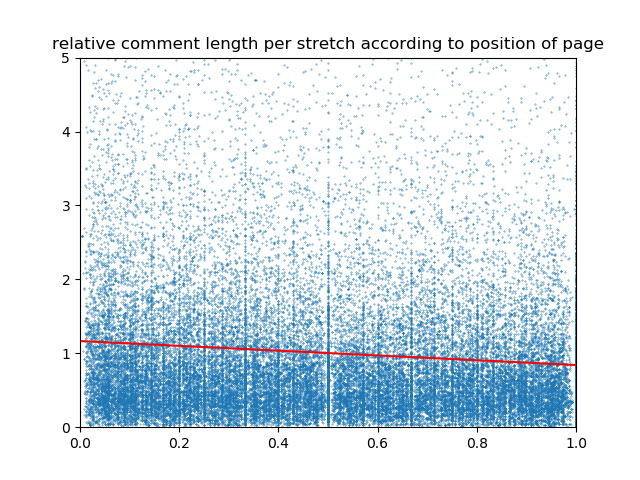
\includegraphics[height=\textheight]{stretchespages.png}
}

\frame{
\frametitle{Ergebnisse für Hypothese \#2\\ ``Ermattung''}
%   \includegraphics[height=.6\textheight]{./path/to/graphicsfile}
  \begin{itemize}
    \item  Die Hypothese ist bestätigt
    \begin{itemize}
      \item je später ein Kommentare im Dokument auftaucht, desto kürzer ist er.
      \item Der erste Kommentar hat im Schnitt 110\% der Durchschnittslänge; der letzte Kommentar 90 \%.
      \item Effekt schwach, aber messbar.
    \end{itemize}
  \end{itemize}
}

\section{Diskussion}
\frame{
\frametitle{Diskussion}
%   \includegraphics[height=.6\textheight]{./path/to/graphicsfile}
  \begin{itemize}
    \item  Wesentliches Ziel ist methodologisch
    \item Kommentare sind ein Nebenprodukt von Open Publishing
    \begin{itemize}
      \item im traditionellen Modell nicht zugänglich 
    \end{itemize}
    \item Wenn Dokumente, Prozesse und Formate geöffnet werden, ergeben sich neue Forschungsfragestellungen, die in traditionellen Abläufen ausgeschlossen waren.  
    \item Eventuell interessant für die Leseforschung. 
  \end{itemize}
}

\section{Das Ökosystem}
\frame{
\frametitle{Nehmen Forschende in der Tat verschiedene Rollen an?}
\begin{columns}
  \begin{column}{5cm}
  \begin{itemize}
    \item  908 Forschende mit Rolle ``author'' bei Language Science Press
    \item 228 Forschende mit Rolle ``proofreader'' 
    \item 27 Forschende in der Schnittmenge
    \begin{itemize}
      \item 16 erst Autor, später Proofreader
      \item 11 erst Proofreader, später Autor
      \item Bewegung in beide Richtungen
      \item Bindung an den Verlag
    \end{itemize}
  \end{itemize}
  \end{column}
  \begin{column}{5cm}
  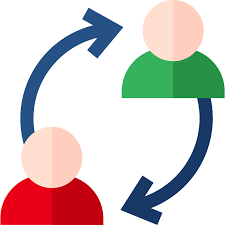
\includegraphics[width=\textwidth]{exchange.png}
  \end{column}
\end{columns}
}

  
\section{Zusammenfassung}
\frame{
\frametitle{Zusammenfassung}
%   \includegraphics[height=.6\textheight]{./path/to/graphicsfile}
  \begin{itemize}
    \item  
Community proofreading ist eine neuer Weg zur Einbindung der Community
    \item 
nur möglich bei OA
\item
nur möglich bei Fachcommunitys (nicht bei Uni-Verlagen)
\item 
Implementation für 50+ Bücher und 200+ Teilnehmer getestet
\item 
vergleichbar mit traditionellem Lektorat/Korrektorat
\item 
Nebenprodukte können für weitere Forschungsfragestellungen verwendet werden
\item Evolution in beide Richtungen Autor {$\leftrightarrow$} Proofreader 
\item Forschende können sich je nach Erfahrung unterschiedlich beteiligen, um Manuskripte zu verbessern
  \end{itemize}
}

\frame{
\frametitle{Fragen}
%   \includegraphics[height=.2\textheight]{./path/to/graphicsfile}
  \begin{itemize}
    \item Welche anderen Fragestellungen könnte man anhand dieser Daten beantworten?
    \item Welche anderen wissenschaftlichen Disziplinen könnten interessiert sein? 
  \end{itemize}
}
\frame{
\frametitle{Vielen Dank}
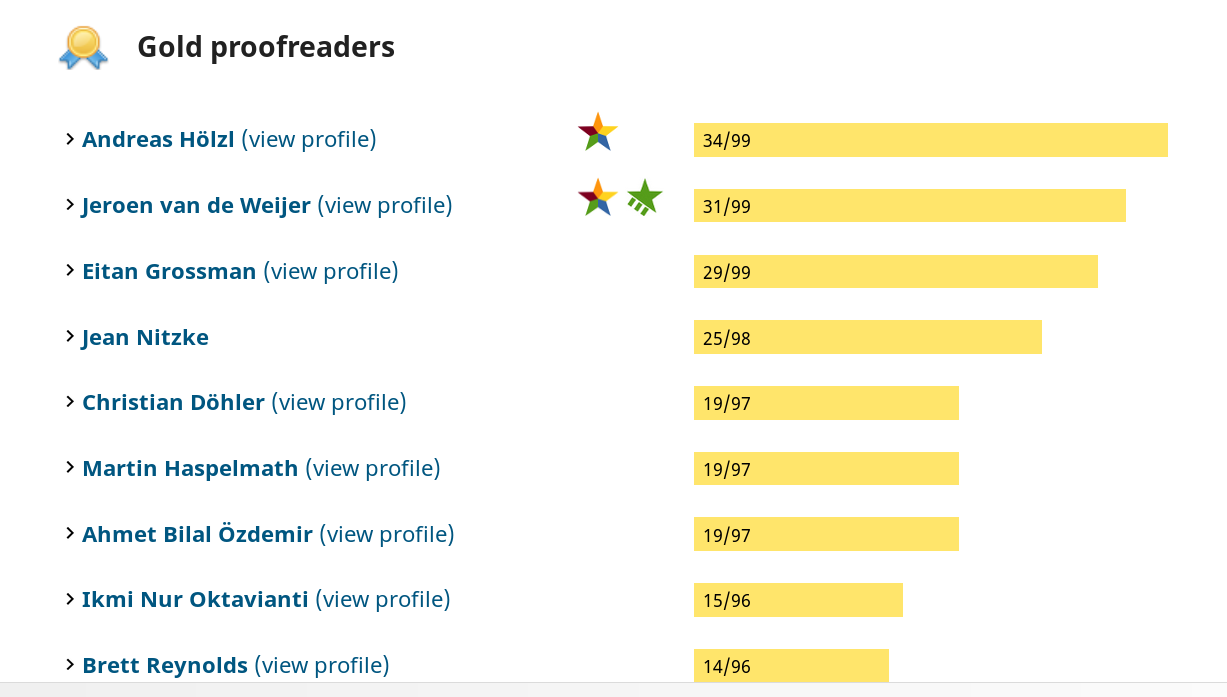
\includegraphics[height=\textheight]{halloffame.png}
}
\end{document}
